\documentclass[hyperref={bookmarks=false},aspectratio=169]{beamer}
\usepackage{hyperref,ragged2e,amsmath,amssymb,url,bm}
\usepackage{graphicx,booktabs,array}
\usepackage{tikz}
\usetikzlibrary{arrows.meta,positioning,calc,shapes.geometric,decorations.pathreplacing,matrix}
\graphicspath{{crops/}}
\usetheme{Goettingen}
% --- Paleta "Israel": café ladrillo (ladrillos de Egipto, Éx 1:14), oro del santuario, piedra de Jerusalén ---
\definecolor{cafe}{RGB}{96,52,30}
\definecolor{cafeosc}{RGB}{50,25,13}
\definecolor{tinta}{RGB}{44,28,18}
\definecolor{oro}{RGB}{196,148,40}
\definecolor{ladrillo}{RGB}{158,70,40}
\definecolor{piedra}{RGB}{240,228,203}
\definecolor{sepia}{RGB}{104,86,62}
\setbeamercolor{structure}{fg=ladrillo}
\setbeamertemplate{sidebar canvas right}[vertical shading][top=ladrillo!92!black,bottom=cafeosc]
\setbeamercolor{title in sidebar}{fg=oro}
\setbeamercolor{author in sidebar}{fg=piedra}
\setbeamercolor{section in sidebar}{fg=piedra}
\setbeamercolor{section in sidebar shaded}{fg=oro!60!piedra!70!cafe}
\setbeamercolor{subsection in sidebar}{fg=piedra}
\setbeamercolor{subsection in sidebar shaded}{fg=oro!60!piedra!70!cafe}
\let\raggedright\justifying
\setbeamertemplate{background canvas}{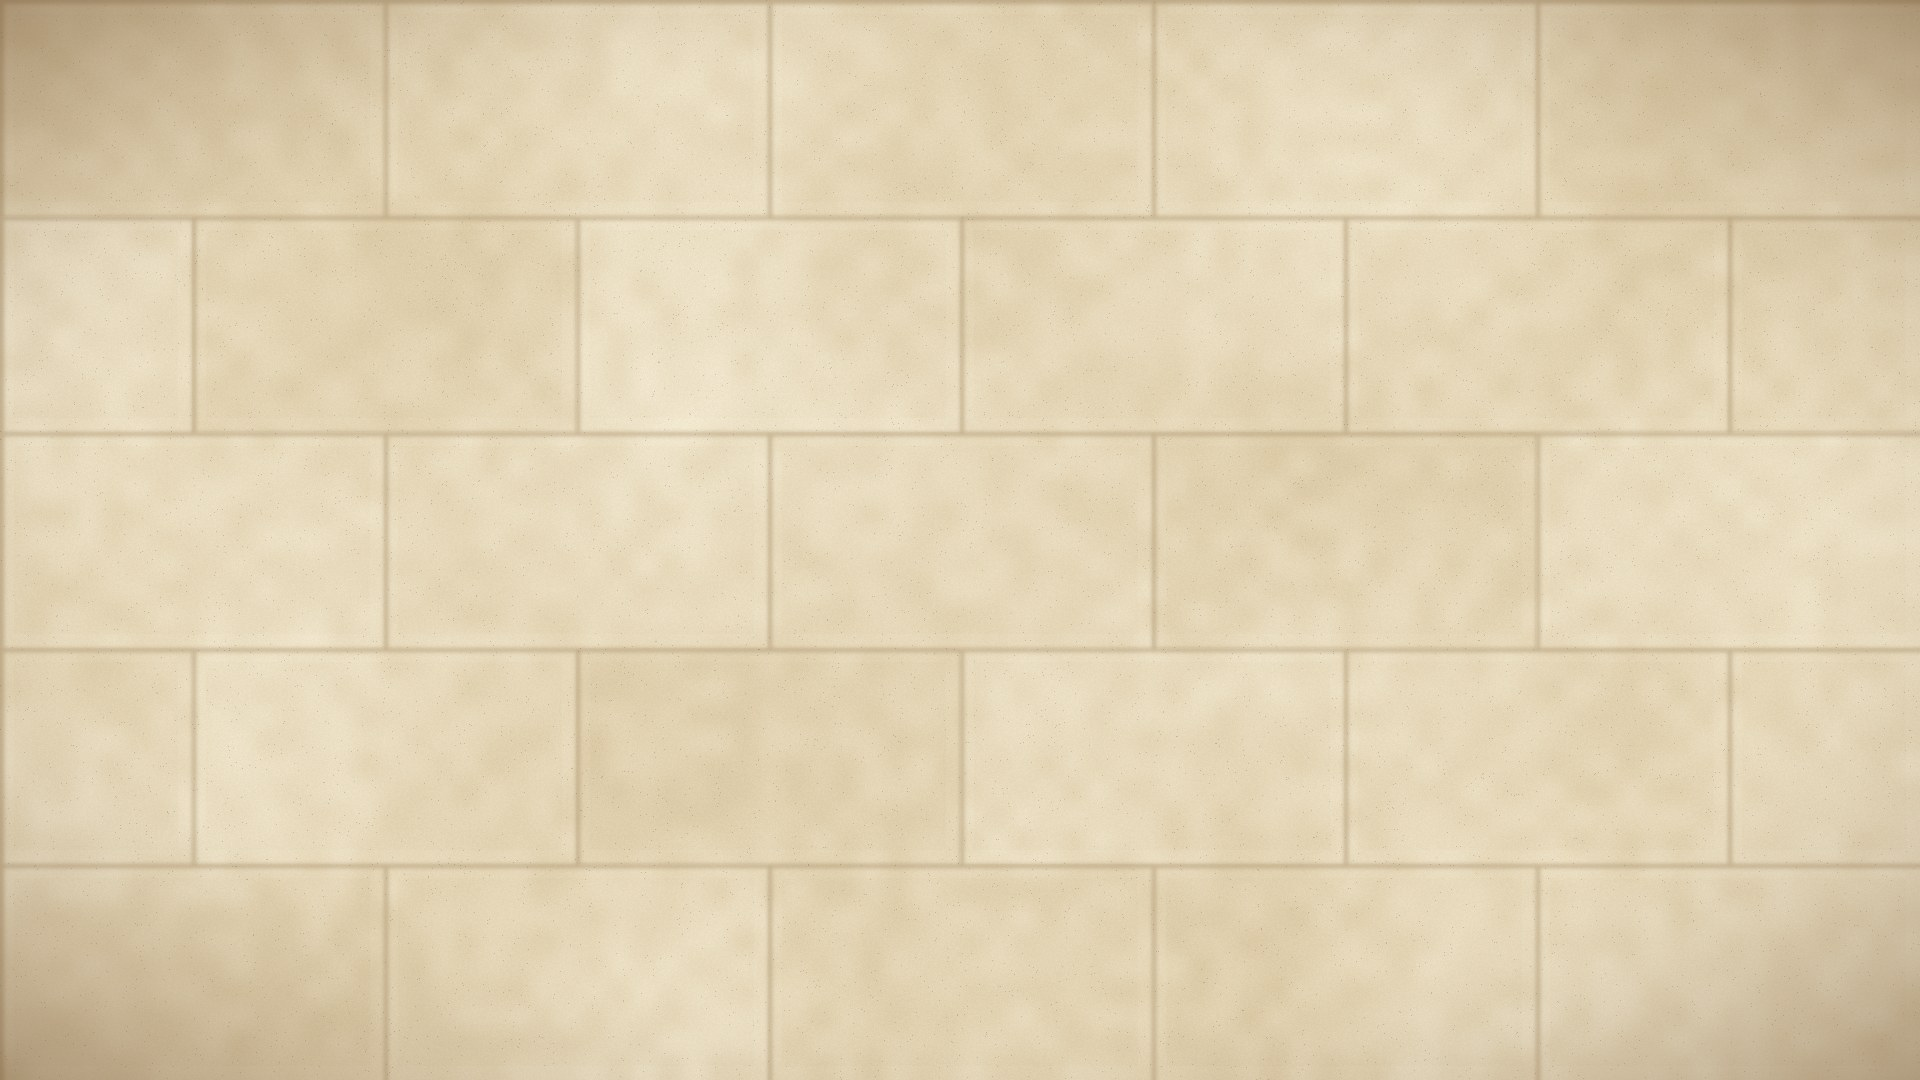
\includegraphics[width=\paperwidth,height=\paperheight]{piedra.jpg}}
\setbeamercolor{normal text}{fg=tinta}
\setbeamercolor{frametitle}{fg=ladrillo}
\setbeamerfont{frametitle}{series=\bfseries}
\setbeamertemplate{section in toc shaded}{\leavevmode{\color{sepia!85!black}\inserttocsection}\par}
\setbeamercolor{title}{fg=ladrillo}
\setbeamercolor{subtitle}{fg=cafe}
\setbeamercolor{item projected}{bg=cafe,fg=piedra}
\setbeamertemplate{itemize item}{\small\textcolor{oro!85!ladrillo}{$\blacktriangleright$}}
\setbeamertemplate{navigation symbols}{}
% --- Español + hebreo + griego (XeLaTeX) con fuentes empaquetadas en fonts/ ---
\usepackage[bidi=default]{babel}
\babelprovide[import,main]{spanish}
\babelprovide[import]{hebrew}
\babelprovide[import]{ancientgreek}
\babelfont[hebrew]{sf}[Path=fonts/, BoldFont=NotoHebrewSans-700.ttf]{NotoHebrewSans-400.ttf}
\babelfont[hebrew]{rm}[Path=fonts/, BoldFont=NotoHebrewSans-700.ttf]{NotoHebrewSans-400.ttf}
\babelfont[ancientgreek]{sf}[Path=fonts/]{GFSPorson.otf}
\babelfont[ancientgreek]{rm}[Path=fonts/]{GFSPorson.otf}
\newcommand{\heb}[1]{\mbox{\foreignlanguage{hebrew}{#1}}}
\newcommand{\grc}[1]{\foreignlanguage{ancientgreek}{#1}}
% --- Citas, imágenes, referencias ---
\usepackage[most]{tcolorbox}
\newtcolorbox{cita}[1][]{enhanced, colback=piedra!92!white, colframe=ladrillo!85!oro,
  boxrule=0pt, leftrule=2.5pt, arc=0pt, left=6pt, right=6pt, top=4pt, bottom=4pt,
  before skip=4pt, after skip=6pt, fontupper=\small\itshape, #1}
\newcommand{\fuente}[1]{\par\hfill{\upshape\bfseries\footnotesize\textcolor{ladrillo}{#1}}}
\newcommand{\imagen}[3][0.80]{%
  \centering\includegraphics[height=#1\textheight,width=\linewidth,keepaspectratio]{#2}\par\vspace{2pt}
  {\fontsize{5}{6}\selectfont\color{sepia}{\raggedleft\textit{Nota.} #3\par}}}
\makeatletter
\newcommand{\fotolado}[2]{%
  \begin{tikzpicture}[remember picture,overlay]
    \node[anchor=north east,inner sep=0pt] (foto) at ([xshift=-\beamer@sidebarwidth]current page.north east)
      {\includegraphics[height=\paperheight]{#1}};
    \node[anchor=south east,inner sep=2pt,text=piedra,fill=cafeosc,fill opacity=0.6,text opacity=1,
      font=\fontsize{4.5}{5.5}\selectfont,align=right,text width=4.2cm] at ([xshift=-3pt,yshift=3pt]foto.south east)
      {\textit{Nota.} #2};
  \end{tikzpicture}}
\makeatother
\newcommand{\refapa}[1]{\par\hangindent=1.2em\hangafter=1\noindent #1\par\vspace{3pt}}
\usepackage{xurl}\urlstyle{same}
\newcommand{\destacar}[1]{\textbf{\textcolor{ladrillo}{#1}}}
\tikzset{caja/.style={draw=cafe,line width=0.8pt,fill=piedra,fill opacity=0.9,text opacity=1,rounded corners=3pt,inner sep=5pt,font=\scriptsize}}
\newcommand{\precision}[1]{{\footnotesize\color{sepia}\textbf{Precisión:} #1}}
\newcommand{\pt}[2]{({#1-30},{#2-29})}
\title[Israel 5: Reyes y cautiverios]{\bfseries{Israel, el pueblo de Dios}}
\subtitle{Estudio 5. Los reyes y los cautiverios}
\author{}\institute{}\date{}
\titlegraphic{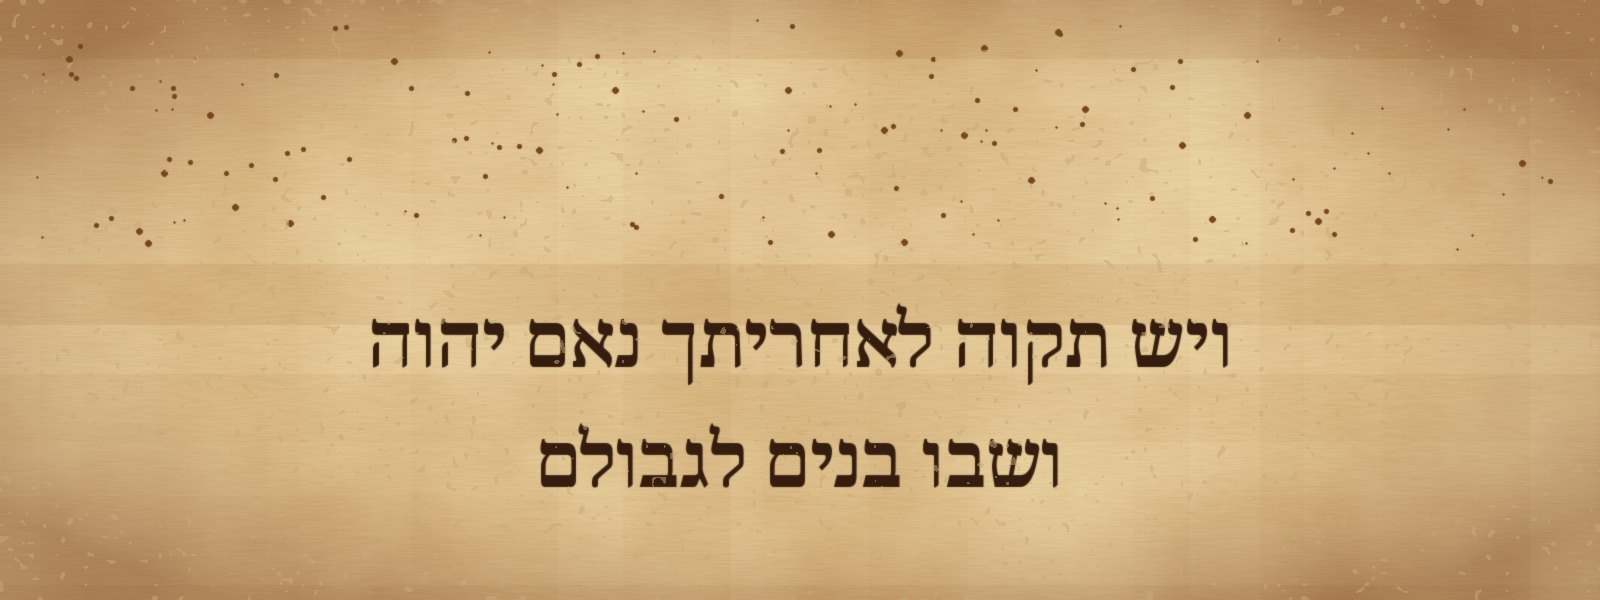
\includegraphics[width=0.85\linewidth,height=0.38\textheight,keepaspectratio]{portada.jpg}\\[-1pt]
  {\fontsize{5}{6}\selectfont\color{sepia}\textit{Nota.} Elaboración propia: Jer 31:17 [31:16] en texto hebreo consonántico (BHS).}}
\AtBeginSection[]{\begin{frame}\frametitle{Contenidos}\tableofcontents[currentsection]\end{frame}}
\newcommand{\X}[1]{(930-#1)*0.0306}
\newcommand{\pq}[2]{({(#1-34.2)*2.25},{(#2-30.95)*2.25})}
\newcommand{\tarjetas}[3]{% #1 alto, #2 ancho, #3 lista x/n/t/d/r
 \begin{tikzpicture}
 \foreach \x/\n/\t/\d/\r in {#3}{
  \node[caja,anchor=north] (b\n) at (\x,0) {\parbox[t][#1][t]{#2}{\RaggedRight
    {\small\textbf{\textcolor{ladrillo}{\t}}}\\[4pt]\scriptsize \d\par\vfill{\tiny\color{sepia}(\r)}}};
  \node[circle,fill=cafe,text=piedra,font=\scriptsize\bfseries,inner sep=1.6pt] at (b\n.north west) {\n};}
 \end{tikzpicture}}
\begin{document}
\frame{\titlepage}
\begin{frame}\frametitle{Contenidos}\tableofcontents\end{frame}

% ===================================================
\section{Introducción}
\begin{frame}{¿Qué queda de Israel?}
\begin{columns}[t,onlytextwidth]
\begin{column}{0.50\textwidth}
\begin{cita}Así fue llevado Israel cautivo de su tierra a Asiria, hasta hoy.\fuente{(2~R 17:23)}\end{cita}
\begin{cita}No ha desechado Dios a su pueblo, al cual antes conoció.\fuente{(Ro 11:2)}\end{cita}
\small Dos veces deja Israel de existir como reino: Samaria en 722 y Jerusalén en 586 a.\,e.\,c.
\end{column}
\begin{column}{0.47\textwidth}\small
\destacar{Tesis 1.} La vocación sacerdotal se quiebra en los dos reinos (idolatría, injusticia, templo como amuleto), pero se preserva en un remanente, en los profetas y en desterrados fieles.\par\medskip
\destacar{Tesis 2.} En la hora del juicio, la promesa de restauración se amplía: remanente que vuelve, nuevo pacto con las dos casas, un solo reino bajo un rey davídico (Jer 31; Ez 37).
\end{column}
\end{columns}
\end{frame}

\begin{frame}{Tres sentidos de «Israel»}
\centering
\tarjetas{2.95cm}{3.55cm}{0/1/{Israel (norte)}/{Diez tribus encabezadas por Efraín; capitales Siquem, Tirsa y Samaria. Los profetas lo llaman «Efraín», «Samaria» o «casa de Israel».}/{1~R 12:16--20; Os 5:3},
   4.2/2/{Judá (sur)}/{Judá y Benjamín, Jerusalén y la casa de David; con levitas y emigrados de otras tribus.}/{1~R 12:21; 2~Cr 11:13--17},
   8.4/3/{Israel (el pueblo)}/{Las doce tribus como pueblo del pacto: «toda la casa de Israel».}/{Jer 31:1; Ez 37:11}}\par\vspace{6pt}
\begin{minipage}{0.95\linewidth}\scriptsize En cada texto se indica qué sentido se usa.\par
{\color{sepia}Las citas bíblicas son traducción propia desde el texto hebreo (BHS) y griego (NA28). Numeración española [hebrea] cuando difiere. Fechas a.\,e.\,c. según Thiele (1983).}\end{minipage}
\end{frame}

% ===================================================
\section{Cronología}
\begin{frame}{Dos reinos, 345 años}
\centering
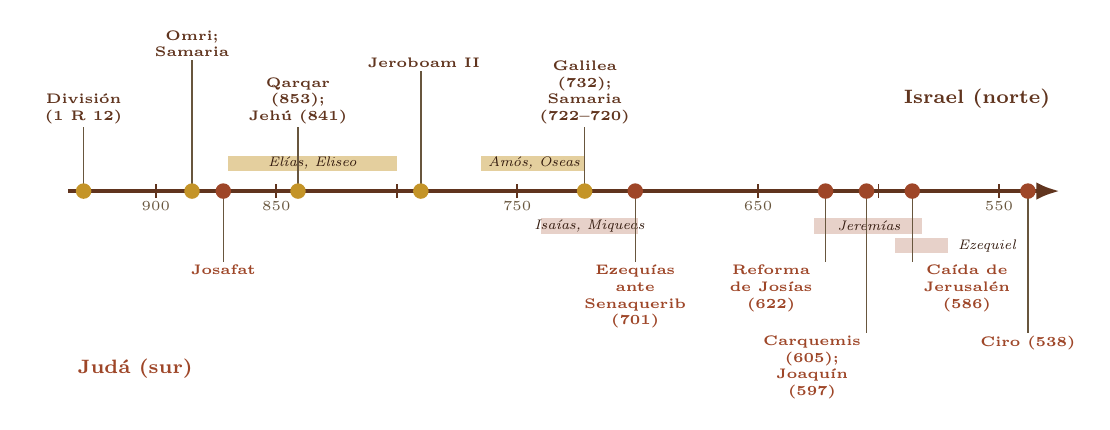
\begin{tikzpicture}[x=1cm,y=0.9cm]
\draw[line width=1.6pt,cafe,-{Latex[length=3mm]}] (-0.2,0) -- (12.4,0);
\foreach \a in {900,850,800,750,700,650,600,550}{\draw[cafe,line width=0.6pt] ({\X{\a}},-0.1) -- ({\X{\a}},0.1);}
\foreach \a in {900,850,750,650,550}{\node[font=\fontsize{4.5}{5}\selectfont,text=sepia,anchor=north,inner sep=1pt] at ({\X{\a}},-0.1) {\a};}
\fill[oro!45] ({\X{870}},0.28) rectangle ({\X{800}},0.5); \node[font=\fontsize{4.5}{5}\selectfont\itshape,text=cafeosc] at ({\X{835}},0.39) {Elías, Eliseo};
\fill[oro!45] ({\X{765}},0.28) rectangle ({\X{722}},0.5); \node[font=\fontsize{4.5}{5}\selectfont\itshape,text=cafeosc] at ({\X{743}},0.39) {Amós, Oseas};
\fill[ladrillo!25] ({\X{740}},-0.38) rectangle ({\X{700}},-0.6); \node[font=\fontsize{4.5}{5}\selectfont\itshape,text=cafeosc] at ({\X{720}},-0.49) {Isaías, Miqueas};
\fill[ladrillo!25] ({\X{627}},-0.38) rectangle ({\X{582}},-0.6); \node[font=\fontsize{4.5}{5}\selectfont\itshape,text=cafeosc] at ({\X{604}},-0.49) {Jeremías};
\fill[ladrillo!25] ({\X{593}},-0.66) rectangle ({\X{571}},-0.88); \node[font=\fontsize{4.5}{5}\selectfont\itshape,text=cafeosc,right] at ({\X{571}},-0.77) {Ezequiel};
\node[font=\scriptsize\bfseries,text=cafe,anchor=east] at (12.4,1.3) {Israel (norte)};
\node[font=\scriptsize\bfseries,text=ladrillo,anchor=west] at (-0.2,-2.5) {Judá (sur)};
\foreach \y/\h/\t in {930/0.9/{División (1~R 12)},885/1.85/{Omri; Samaria},841/0.9/{Qarqar (853); Jehú (841)},790/1.7/{Jeroboam~II},722/0.9/{Galilea (732); Samaria (722--720)}}{
  \draw[sepia,line width=0.5pt] ({\X{\y}},0) -- ({\X{\y}},\h);
  \fill[oro] ({\X{\y}},0) circle (2.8pt);
  \node[above,font=\fontsize{5}{6}\selectfont\bfseries,text=cafe,text width=1.35cm,align=center,inner sep=1pt] at ({\X{\y}},\h) {\t};}
\foreach \y/\h/\an/\t in {872/1.0/north/{Josafat},701/1.0/north/{Ezequías ante Senaquerib (701)},622/1.0/north east/{Reforma de Josías (622)},605/2.0/north east/{Carquemis (605); Joaquín (597)},586/1.0/north west/{Caída de Jerusalén (586)},538/2.0/north/{Ciro (538)}}{
  \draw[sepia,line width=0.5pt] ({\X{\y}},0) -- ({\X{\y}},-\h);
  \fill[ladrillo] ({\X{\y}},0) circle (2.8pt);
  \node[anchor=\an,font=\fontsize{5}{6}\selectfont\bfseries,text=ladrillo,text width=1.3cm,align=center,inner sep=1pt] at ({\X{\y}},-\h) {\t};}
\end{tikzpicture}\par\vspace{2pt}
{\fontsize{5}{6}\selectfont\color{sepia}\raggedleft\textit{Nota.} Elaboración propia. Fechas aproximadas (Thiele, 1983); bandas: actividad de los profetas.\par}
\end{frame}

\begin{frame}{Dos reinos en el mapa}
\begin{columns}[c,onlytextwidth]
\begin{column}{0.44\textwidth}
\centering
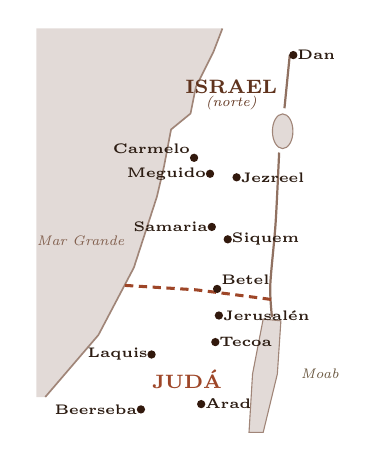
\begin{tikzpicture}
\fill[cafe!18] \pq{34.2}{31.32} -- \pq{34.25}{31.32} -- \pq{34.55}{31.67} -- \pq{34.75}{32.05} -- \pq{34.88}{32.45} -- \pq{34.92}{32.62} -- \pq{34.96}{32.83} -- \pq{35.07}{32.92} -- \pq{35.10}{33.07} -- \pq{35.20}{33.27} -- \pq{35.25}{33.4} -- \pq{34.2}{33.4} -- cycle;
\draw[cafe!60,line width=0.6pt] \pq{34.25}{31.32} -- \pq{34.55}{31.67} -- \pq{34.75}{32.05} -- \pq{34.88}{32.45} -- \pq{34.92}{32.62} -- \pq{34.96}{32.83} -- \pq{35.07}{32.92} -- \pq{35.10}{33.07} -- \pq{35.20}{33.27} -- \pq{35.25}{33.4};
\fill[cafe!18,draw=cafe!60] \pq{35.48}{31.76} -- \pq{35.58}{31.75} -- \pq{35.56}{31.45} -- \pq{35.48}{31.12} -- \pq{35.40}{31.12} -- \pq{35.42}{31.45} -- cycle;
\fill[cafe!18,draw=cafe!60] \pq{35.59}{32.82} ellipse (0.13 and 0.22);
\draw[cafe!70,line width=0.8pt] plot[smooth] coordinates {\pq{35.63}{33.25} \pq{35.6}{32.95}};
\draw[cafe!70,line width=0.8pt] plot[smooth] coordinates {\pq{35.57}{32.70} \pq{35.55}{32.3} \pq{35.52}{31.95} \pq{35.53}{31.77}};
\draw[ladrillo,line width=1.1pt,dash pattern=on 3pt off 2pt] \pq{34.70}{31.95} -- \pq{35.1}{31.925} -- \pq{35.30}{31.90} -- \pq{35.53}{31.87};
\node[font=\scriptsize\bfseries,text=cafe] at \pq{35.3}{33.07} {ISRAEL};
\node[font=\tiny\itshape,text=cafe] at \pq{35.3}{32.98} {(norte)};
\node[font=\scriptsize\bfseries,text=ladrillo] at \pq{35.05}{31.42} {JUDÁ};
\node[font=\tiny\itshape,text=cafe!80] at \pq{34.45}{32.2} {Mar Grande};
\node[font=\tiny\itshape,text=sepia] at \pq{35.8}{31.45} {Moab};
\foreach \lon/\lat/\n/\p in {35.65/33.25/Dan/right, 35.19/32.28/Samaria/left, 35.28/32.21/Siquem/right, 35.33/32.56/Jezreel/right, 35.18/32.58/Meguido/left, 35.09/32.67/Carmelo/above left, 35.22/31.93/Betel/above right, 35.23/31.78/Jerusalén/right, 34.85/31.56/Laquis/left, 35.21/31.63/Tecoa/right, 35.13/31.28/Arad/right, 34.79/31.25/Beerseba/left}{
  \fill[cafeosc] \pq{\lon}{\lat} circle (1.5pt);
  \node[\p,font=\tiny\bfseries,text=tinta,inner sep=1.3pt] at \pq{\lon}{\lat} {\n};}
\end{tikzpicture}\\
{\fontsize{5}{6}\selectfont\color{sepia}\textit{Nota.} Elaboración propia: esquema con coordenadas reales; frontera aproximada.}
\end{column}
\begin{column}{0.54\textwidth}\scriptsize
\renewcommand{\arraystretch}{1.15}
\begin{tabular}{>{\RaggedRight\arraybackslash}p{2.75cm}>{\RaggedRight\arraybackslash}p{3.05cm}}
\toprule
\textbf{Israel (norte)} & \textbf{Judá}\\\midrule
9 dinastías, 19 reyes; 7 asesinados & 1 dinastía (David), 19 reyes y Atalía\\
Jeroboam~I (931--910) & Roboam (931--913); Asa\\
Omri (885--874), Acab & Josafat (872--848)\\
Jehú (841--814) & Joás; Uzías (792--740)\\
Jeroboam~II (793--753) & Acaz; Ezequías (715--686)\\
Manahem; Peka & Manasés (697--642)\\
Oseas (732--722) & Josías (640--609)\\
--- & Joacim, Joaquín, Sedequías (609--586)\\
\bottomrule
\end{tabular}\par\smallskip
La promesa a David sostiene a Judá aun bajo reyes infieles, «por amor a David mi siervo» (1~R 11:13; 2~R 8:19).
\end{column}
\end{columns}
\end{frame}

% ===================================================
\section{Arqueología}
\begin{frame}{El reino del norte en piedra}
\centering
\tarjetas{3.25cm}{2.65cm}{0/1/{Estela de Mesa}/{«Omri era rey de Israel y oprimió a Moab muchos días». Menciona a YHWH (cf. 2~R 3:4--5).}/{c. 840; Louvre},
   3.15/2/{Monolito de Kurkh}/{«Acab el israelita» en Qarqar con 2.000 carros, el mayor contingente de la coalición.}/{853; Salmanasar III},
   6.3/3/{Obelisco Negro}/{«Jehú, hijo de Omri», postrado ante el rey asirio. «Hijo de Omri» designa al reino.}/{841; Museo Británico},
   9.45/4/{Sargón II}/{«Sitié y conquisté Samaria; llevé cautivos a 27.290 habitantes» y la repoblé (cf. 2~R 17:24).}/{Jorsabad; Nimrud: 27.280}}\par\vspace{5pt}
\begin{minipage}{0.95\linewidth}\scriptsize También: \textbf{Tel Dan} (un rey arameo dice haber matado a [Jo]ram de Israel y a [Ocoz]ías de la «casa de David»; cf. 2~R 9); \textbf{Tiglat-pileser~III} («derrocaron a Peka y puse a Oseas», cf. 2~R 15:29--30); \textbf{ostracones de Samaria} (s. \textsc{viii}: nombres con \emph{-yau} y con Baal; cf. Os 2:16--17 [2:18--19]).\end{minipage}
\end{frame}

\begin{frame}{Judá ante Asiria}
\centering
\tarjetas{3.25cm}{2.65cm}{0/1/{Prisma de Senaquerib}/{46 ciudades tomadas; Ezequías encerrado «como un pájaro en su jaula». No dice haber tomado Jerusalén.}/{701; cf. 2~R 18:13--19:36},
   3.15/2/{Relieves de Laquis}/{El asedio en piedra en Nínive; en Laquis, la rampa asiria y el estrato destruido.}/{Ussishkin, 1982},
   6.3/3/{Túnel de Siloé}/{Unos 533 m desde Guijón; la inscripción narra el encuentro de las cuadrillas. Datación c. 700.}/{2~R 20:20; Frumkin et al., 2003},
   9.45/4/{Bulas y amuletos}/{«De Ezequías [hijo de] Acaz, rey de Judá». Ketef Hinom: Nm 6:24--26 en plata.}/{Barkay et al., 2004}}\par\vspace{5pt}
\begin{minipage}{0.95\linewidth}\precision{la bula «Yesha\textquoteright yah[u] \emph{nby}» se ha propuesto como del profeta Isaías (Mazar, 2018), pero falta la última letra y la lectura es discutida.}\end{minipage}
\end{frame}

\begin{frame}{Judá ante Babilonia}
\centering
\tarjetas{3.25cm}{2.65cm}{0/1/{Crónica babilónica}/{Carquemis (605). «El 2 de Adar tomó la ciudad de Judá, capturó al rey y nombró uno de su elección».}/{16 mar. 597; Grayson, 1975},
   3.15/2/{Tablillas de Weidner}/{Raciones de aceite para «Ya\textquoteright ukinu, rey de Yahudu», y sus cinco hijos.}/{c. 592; cf. 2~R 25:27--30},
   6.3/3/{Cartas de Laquis}/{«Estamos atentos a las señales de Laquis [\ldots] porque no vemos Azeca».}/{c. 588; cf. Jer 34:7},
   9.45/4/{Estrato de 586}/{Casas quemadas, puntas de flecha; bula de «Gemaryahu hijo de Safán».}/{Shiloh, 1986; cf. Jer 36:10}}\par\vspace{5pt}
\begin{minipage}{0.95\linewidth}\scriptsize \textbf{Al-Yahudu} (c. 572--477): contratos de una aldea babilónica llamada «ciudad de Judá», con nombres yahvistas durante generaciones (Pearce y Wunsch, 2014): los desterrados «edificaron casas y plantaron huertos» (Jer 29:5).\end{minipage}
\end{frame}

% ===================================================
\section{El norte}
\begin{frame}{Un trono sin pacto}
\begin{columns}[t,onlytextwidth]
\begin{column}{0.50\textwidth}
\begin{cita}He aquí tus dioses, oh Israel, que te hicieron subir de la tierra de Egipto.\fuente{(1~R 12:28; cf. Éx 32:4)}\end{cita}
\small Jeroboam levanta becerros en Betel y Dan, nombra sacerdotes no levitas y cambia el calendario (1~R 12:28--33). «El pecado de Jeroboam» será el estribillo de Reyes.
\end{column}
\begin{column}{0.47\textwidth}\small
\textbf{\textcolor{cafe}{Migraciones al sur}}
\begin{itemize}
\item Bajo Roboam: sacerdotes, levitas y fieles «de todas las tribus» (2~Cr 11:13--16).
\item Bajo Asa: de Efraín, Manasés y Simeón (2~Cr 15:9).
\end{itemize}
\precision{desde el inicio, Judá reúne fieles de todas las tribus (Departamento de Educación, s.\,f.-a, diap. 13).}
\end{column}
\end{columns}
\end{frame}

\begin{frame}{El Carmelo y los siete mil}
\fotolado{panel_1r19.jpg}{Elaboración propia: 1~R 19:18 en texto hebreo consonántico (BHS).}
\begin{columns}[c,onlytextwidth]
\begin{column}{0.57\textwidth}
\small «¿Hasta cuándo saltaréis entre dos ramas?» (1~R 18:21). Elías reconstruye el altar con \destacar{doce piedras}, una por tribu (18:31): aun en el norte, Israel es un pueblo de doce tribus.
\begin{cita}Haré que queden en Israel siete mil: todas las rodillas que no se doblaron ante Baal.\fuente{(1~R 19:18)}\end{cita}
\scriptsize
\begin{itemize}
\item \heb{וְהִשְׁאַרְתִּי} (\emph{ve-hish'arti}): hifil causativo: el remanente existe porque Dios lo deja.
\item Raíz de \heb{שְׁאָר} y \heb{שְׁאֵרִית}, «remanente».
\end{itemize}
\end{column}
\begin{column}{0.41\textwidth}\end{column}
\end{columns}
\end{frame}

\begin{frame}{Del Horeb a Romanos 11}
\centering
\begin{tikzpicture}[node distance=0.85cm]
\node[caja,text width=3.3cm,align=center] (h) {\textbf{1 R 19:18 (TM)}\\[3pt]\heb{וְהִשְׁאַרְתִּי}\\[2pt]«haré que queden»\\[1pt]\heb{לַבַּעַל}};
\node[caja,text width=3.3cm,align=center,right=of h] (g) {\textbf{LXX (3 Re 19:18)}\\[3pt]\grc{καταλείψεις}\\[2pt]\grc{τῷ Βααλ}\\[1pt](artículo masculino)};
\node[caja,text width=3.3cm,align=center,right=of g] (p) {\textbf{Pablo (Ro 11:4--5)}\\[3pt]\grc{κατέλιπον ἐμαυτῷ}\\[2pt]\grc{τῇ Βάαλ}\\[1pt]\grc{λεῖμμα κατ᾽ ἐκλογὴν χάριτος}};
\draw[-{Latex[length=2.5mm]},oro!90!ladrillo,line width=1.4pt] (h) -- (g);
\draw[-{Latex[length=2.5mm]},oro!90!ladrillo,line width=1.4pt] (g) -- (p);
\end{tikzpicture}\par\vspace{6pt}
\begin{cita}Así también, en el tiempo presente, ha quedado un remanente escogido por gracia.\fuente{(Ro 11:5)}\end{cita}
\begin{minipage}{0.95\linewidth}\precision{el femenino \grc{τῇ Βάαλ} quizá refleja la lectura \grc{αἰσχύνη}, «vergüenza», en lugar del ídolo (cf. Is-boset, 2~S 2:8). Hipótesis, no demostrada (Moo, 1996).}\end{minipage}
\end{frame}

\begin{frame}{Eliseo, Jehú y Jeroboam II}
\begin{columns}[t,onlytextwidth]
\begin{column}{0.48\textwidth}\small
\begin{itemize}
\item \textbf{Eliseo}: Naamán el arameo confiesa que «no hay Dios en toda la tierra sino en Israel» (2~R 5:15; Lc 4:27).
\item \textbf{Jehú}: extermina la casa de Acab y el culto a Baal, pero conserva los becerros (2~R 10:29); Oseas anuncia juicio por «la sangre de Jezreel» (Os 1:4).
\item \textbf{Jeroboam~II}: máxima extensión del norte, según Jonás hijo de Amitai (2~R 14:25).
\end{itemize}
\end{column}
\begin{column}{0.49\textwidth}
\centering{\heb{וְלֹא־דִבֶּר יְהוָה לִמְחוֹת}}\\[-1pt]{\heb{אֶת־שֵׁם יִשְׂרָאֵל מִתַּחַת הַשָּׁמָיִם}}\par\smallskip
\begin{cita}Y YHWH no había dicho que borraría el nombre de Israel de debajo del cielo.\fuente{(2~R 14:27)}\end{cita}
\small Aquí «Israel» es el reino del norte. La prosperidad se explica por la misericordia, no por el mérito.
\end{column}
\end{columns}
\end{frame}

\begin{frame}{Amós y Oseas: «no mi pueblo»}
\begin{columns}[t,onlytextwidth]
\begin{column}{0.48\textwidth}\small
\textbf{\textcolor{cafe}{Amós}} (de Tecoa, en Betel): «solo a vosotros he conocido [\ldots]; por eso os castigaré» (Am 3:2). Zarandeados entre las naciones, «no caerá un grano a tierra» (9:9).\par\medskip
\textbf{\textcolor{cafe}{Oseas}}: Jezreel, Lo-Ruhamá, \destacar{Lo-Ammí}.
\centering{\heb{כִּי אַתֶּם לֹא עַמִּי וְאָנֹכִי לֹא־אֶהְיֶה לָכֶם}}\par
\RaggedRight\scriptsize «No sois mi pueblo, y yo no seré vuestro» (Os 1:9): \heb{לֹא־אֶהְיֶה} niega el \heb{אֶהְיֶה} de Éx 3:14.
\end{column}
\begin{column}{0.49\textwidth}
\begin{cita}[fontupper=\scriptsize\itshape]En el lugar donde se les dijo: «No sois mi pueblo», se les dirá: «Hijos del Dios viviente». Y se reunirán los hijos de Judá y los hijos de Israel, y se pondrán una sola cabeza.\fuente{(Os 1:10--11 [2:1--2])}\end{cita}
\scriptsize
\begin{itemize}
\item La cabeza: «David su rey [\ldots] al fin de los días» (Os 3:5).
\item Pablo cita Oseas en Ro 9:25--26 y lo aplica a los llamados «también de los gentiles» (9:24): lectura analógica (Moo, 1996).
\end{itemize}
\end{column}
\end{columns}
\end{frame}

\begin{frame}{La caída de Samaria}
\begin{columns}[c,onlytextwidth]
\begin{column}{0.64\textwidth}
\centering
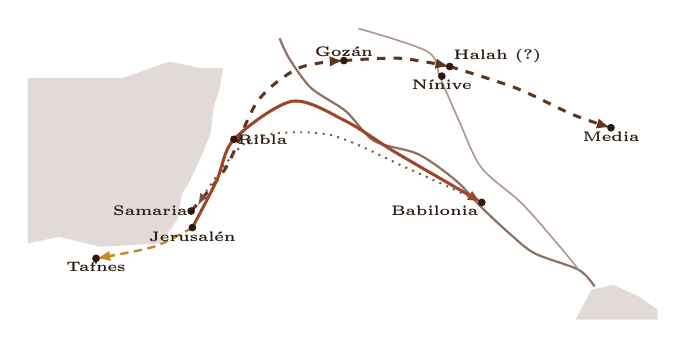
\begin{tikzpicture}[x=0.4cm,y=0.42cm]
\fill[cafe!18] (0,2.3) -- \pt{31.0}{31.5} -- \pt{32.3}{31.2} -- \pt{34.2}{31.3} -- \pt{34.75}{32.0} -- \pt{34.9}{32.8} -- \pt{35.1}{33.1} -- \pt{35.5}{33.9} -- \pt{35.8}{34.6} -- \pt{35.9}{35.4} -- \pt{36.1}{36.0} -- \pt{36.2}{36.6} -- \pt{35.5}{36.6} -- \pt{34.5}{36.8} -- \pt{33}{36.3} -- (0,7.3) -- cycle;
\fill[cafe!18] \pt{47.4}{29.0} -- \pt{47.9}{29.9} -- \pt{48.6}{30.05} -- \pt{49.4}{29.7} -- \pt{50}{29.3} -- \pt{50}{29.0} -- cycle;
\draw[cafe!70,line width=0.8pt] plot[smooth] coordinates {\pt{38.0}{37.5} \pt{38.3}{36.9} \pt{39.0}{36.0} \pt{40.1}{35.3} \pt{41.0}{34.4} \pt{42.4}{34.0} \pt{43.6}{33.2} \pt{44.4}{32.4} \pt{45.3}{31.6} \pt{46.1}{31.0} \pt{47.5}{30.5} \pt{48.0}{30.0}};
\draw[cafe!50,line width=0.6pt] plot[smooth] coordinates {\pt{40.5}{37.8} \pt{42.7}{37.1} \pt{43.1}{36.3} \pt{43.7}{35.0} \pt{44.4}{33.6} \pt{45.7}{32.5} \pt{46.9}{31.2} \pt{47.5}{30.5}};
\draw[cafe,line width=1.1pt,dashed,-{Latex[length=1.8mm]}] plot[smooth] coordinates {\pt{35.19}{32.28} \pt{36.3}{33.6} \pt{37.3}{35.6} \pt{38.6}{36.6} \pt{40.04}{36.83}};
\draw[cafe,line width=1.1pt,dashed,-{Latex[length=1.8mm]}] plot[smooth] coordinates {\pt{40.04}{36.83} \pt{41.8}{36.9} \pt{43.4}{36.65}};
\draw[cafe,line width=1.1pt,dashed,-{Latex[length=1.8mm]}] plot[smooth] coordinates {\pt{43.4}{36.65} \pt{45.5}{36.0} \pt{47.3}{35.2} \pt{48.52}{34.8}};
\draw[sepia,line width=0.7pt,dotted,-{Latex[length=1.5mm]}] plot[smooth] coordinates {\pt{44.42}{32.54} \pt{42.0}{33.6} \pt{39.5}{34.6} \pt{37.0}{34.4} \pt{35.4}{32.45}};
\draw[ladrillo,line width=1.1pt,-{Latex[length=1.8mm]}] plot[smooth] coordinates {\pt{35.23}{31.78} \pt{36.0}{33.2} \pt{36.55}{34.45} \pt{38.4}{35.6} \pt{40.1}{35.0} \pt{41.6}{34.1} \pt{43.4}{33.1} \pt{44.42}{32.54}};
\draw[oro!90!ladrillo,line width=0.9pt,densely dashed,-{Latex[length=1.8mm]}] plot[smooth] coordinates {\pt{35.23}{31.78} \pt{34.0}{31.2} \pt{32.17}{30.85}};
\foreach \lon/\lat/\n/\p in {35.19/32.28/Samaria/left, 35.23/31.78/Jerusalén/below, 36.55/34.45/Ribla/right, 40.04/36.83/Gozán/above, 43.15/36.36/Nínive/below, 43.4/36.65/Halah (?)/above right, 48.52/34.8/Media/below, 44.42/32.54/Babilonia/below left, 32.17/30.85/Tafnes/below}{
  \fill[cafeosc] \pt{\lon}{\lat} circle (1.4pt);
  \node[\p,font=\fontsize{4.5}{5}\selectfont\bfseries,text=tinta,inner sep=1.2pt] at \pt{\lon}{\lat} {\n};}
\end{tikzpicture}\\[1pt]
{\fontsize{4.5}{5.5}\selectfont\color{sepia}\textcolor{cafe}{- - -} Asiria (2~R 17:6) \quad \textcolor{sepia}{$\cdots$} colonos a Samaria (17:24) \quad \textcolor{ladrillo}{---} Babilonia (2~R 25) \quad \textcolor{oro!90!ladrillo}{- -} Egipto (Jer 43)\par
\textit{Nota.} Elaboración propia: esquema con coordenadas reales; ubicación de Halah incierta.}
\end{column}
\begin{column}{0.34\textwidth}
\begin{cita}[fontupper=\scriptsize\itshape]El rey de Asiria tomó Samaria y llevó a Israel cautivo a Asiria, y los puso en Halah, en el Habor, río de Gozán, y en las ciudades de los medos.\fuente{(2~R 17:6)}\end{cita}
\scriptsize Fases: Galilea y Galaad (733--732; 2~R 15:29); Samaria (722--720).\par\smallskip
\precision{los 27.290 de Sargón son de Samaria; la población del norte (c. 350.000) y el 10--15 \% deportado son estimaciones (Broshi y Finkelstein, 1992).}
\end{column}
\end{columns}
\end{frame}

\begin{frame}{El sermón de 2 Reyes 17:7--23}
\centering\scriptsize\renewcommand{\arraystretch}{1.18}
\begin{tabular}{>{\RaggedRight\arraybackslash}p{1.35cm}>{\RaggedRight\arraybackslash}p{5.0cm}>{\RaggedRight\arraybackslash}p{4.6cm}}
\toprule
\textbf{Vv.} & \textbf{Contenido} & \textbf{Observación}\\\midrule
17:7--12 & Pecaron contra YHWH, «que los sacó de Egipto»: lugares altos, aseras, ídolos & El destierro invierte el Éxodo\\
17:13 & Amonestó «a Israel y a Judá»: «Volveos (\heb{שֻׁבוּ}) de vuestros malos caminos» & Judá incluido desde ya\\
17:14--17 & «Siguieron la vanidad y se hicieron vanos» (\heb{הַהֶבֶל וַיֶּהְבָּלוּ}) & Uno se vuelve lo que adora (Jer 2:5)\\
17:18 & «No quedó sino solo la tribu de Judá» & Judá con Benjamín y emigrados\\
17:19--20 & «Tampoco Judá guardó [\ldots]»; desechó a «toda la descendencia de Israel» & Aquí «Israel» = el pueblo completo\\
17:21--23 & El pecado de Jeroboam; «llevado cautivo [\ldots] hasta hoy» & La palabra profética se cumplió\\
\bottomrule
\end{tabular}\par\vspace{6pt}
\begin{minipage}{0.95\linewidth}\small El sermón, escrito para judaítas en el exilio, mira hacia Judá. La palabra decisiva es \emph{shuv}, «volverse»: el verbo del regreso.\end{minipage}
\end{frame}

\begin{frame}{Repoblamiento y samaritanos}
\begin{columns}[t,onlytextwidth]
\begin{column}{0.48\textwidth}
\begin{cita}[fontupper=\scriptsize\itshape]El rey de Asiria trajo gente de Babilonia, de Cuta, de Ava, de Hamat y de Sefarvaim, y la puso en las ciudades de Samaria en lugar de los hijos de Israel.\fuente{(2~R 17:24)}\end{cita}
\small «Temían a YHWH y servían a sus dioses» (17:33; cf. Esd 4:2, 10).
\end{column}
\begin{column}{0.49\textwidth}\small
\begin{itemize}
\item \textbf{Tradición judía}: \emph{kutim}, «cuteos» (Josefo, \emph{Ant.} 9.14.3).
\item \textbf{Los samaritanos}: \emph{shamerim}, «guardianes», descendientes de Efraín y Manasés.
\item \textbf{Investigación}: hubo colonos, pero gran parte del norte rural permaneció (Knoppers, 2013).
\item \textbf{NT}: extranjeros (Lc 17:18) y herederos de Jacob (Jn 4:12); reciben el evangelio (Hch 8).
\end{itemize}
\end{column}
\end{columns}
\end{frame}

\begin{frame}{¿Se perdieron las diez tribus?}
\begin{columns}[t,onlytextwidth]
\begin{column}{0.49\textwidth}\scriptsize
\textbf{\small\textcolor{cafe}{Lo que dicen los textos}}
\begin{itemize}
\item Ezequías invita al «remanente que ha quedado de la mano de los reyes de Asiria»; vienen de Aser, Manasés, Zabulón e Isacar (2~Cr 30:6--18).
\item Josías recibe ofrendas de «todo el remanente de Israel» (2~Cr 34:9); tras 586, hombres de Siquem, Silo y Samaria (Jer 41:5).
\item En Jerusalén: Judá, Benjamín, \destacar{Efraín y Manasés} (1~Cr 9:3); doce machos cabríos (Esd 6:17).
\item Ana, «de la tribu de Aser» (Lc 2:36); «nuestras doce tribus» (Hch 26:7).
\end{itemize}
\end{column}
\begin{column}{0.49\textwidth}\scriptsize
\textbf{\small\textcolor{cafe}{Lo que dicen otras fuentes}}
\begin{itemize}
\item Josefo: las diez tribus están «más allá del Éufrates» (\emph{Ant.} 11.5.2). Tobit y 4~Esdras 13: memoria literaria, no crónica.
\item Arqueología: Galilea despoblada tras 732; más continuidad en Samaria (Becking, 1992); israelitas en el ejército de Sargón (Dalley, 1985).
\item Jerusalén crece de 10--12 a c. 60 ha: ¿refugiados del norte (Broshi, 1974; Finkelstein, 2008) o de la Sefelá tras 701 (Na'aman, 2007)?
\end{itemize}
\precision{Neh 11:1--3 nombra solo a Judá, Benjamín, sacerdotes y levitas; los ostracones de Samaria son anteriores a 722.}
\end{column}
\end{columns}
\end{frame}

\begin{frame}{La teoría de las Dos Casas}
\centering\scriptsize\renewcommand{\arraystretch}{1.18}
\begin{tabular}{>{\RaggedRight\arraybackslash}p{2.8cm}>{\RaggedRight\arraybackslash}p{3.4cm}>{\RaggedRight\arraybackslash}p{4.6cm}}
\toprule
\textbf{Argumento} & \textbf{Lo que el texto sí dice} & \textbf{Dificultad}\\\midrule
Las diez tribus se perdieron & Deportación parcial (2~R 17:6) & Muchos quedaron o se unieron a Judá (2~Cr 11; 30; 34; 1~Cr 9:3)\\
\emph{Melo ha-goyim} = «plenitud de los gentiles» & Gn 48:19: \heb{מְלֹא־הַגּוֹיִם}, «multitud de naciones» & LXX: \grc{πλῆθος ἐθνῶν}, no \grc{πλήρωμα}; en Ro 11:13, 25 \grc{ἔθνη} = no israelitas\\
Os 2:1 en Ro 9:25--26 & Pablo aplica Oseas a gentiles & Inclusión por llamado y fe (Ro 9:24, 30), no por genealogía\\
Ez 37; Jer 31:31 & Reunión explícita de dos casas & Ez 37:22: «en la tierra»; Jer 31:33: una sola «casa de Israel»\\
Efraín hoy & --- & Sin evidencia para identificar poblaciones gentiles como Efraín (diap. 22)\\
\bottomrule
\end{tabular}\par\vspace{5pt}
\begin{minipage}{0.95\linewidth}\scriptsize\textbf{Balance}: la promesa de reunir a las dos casas es bíblica; la identificación genealógica de los gentiles con Efraín no tiene apoyo suficiente. \emph{Todo Israel} (Ro 11:26): Estudio~8.\par
{\fontsize{5}{6}\selectfont\color{sepia}Fuente: Departamento de Educación (s.\,f.-b), diapositivas 16--22, con evaluación propia.}\end{minipage}
\end{frame}

% ===================================================
\section{Judá}
\begin{frame}{Josafat y Ezequías}
\begin{columns}[t,onlytextwidth]
\begin{column}{0.46\textwidth}\small
\textbf{\textcolor{cafe}{Josafat}} (872--848): levitas que enseñan «el libro de la ley» (2~Cr 17:7--9); su alianza con Acab trae a Atalía, que casi extingue la casa de David (2~R 11).\par\medskip
\textbf{\textcolor{cafe}{Ezequías}} (715--686): purifica el templo, rompe la serpiente de bronce y \destacar{invita al norte a la Pascua} (2~Cr 30).
\end{column}
\begin{column}{0.51\textwidth}
\begin{cita}[fontupper=\scriptsize\itshape]Sálvanos de su mano, para que sepan todos los reinos de la tierra que solo tú, YHWH, eres Dios.\fuente{(Is 37:20)}\end{cita}
\scriptsize Una oración sacerdotal: Jerusalén salvada para que las naciones conozcan a Dios. Isaías responde: «el remanente de la casa de Judá [\ldots] echará raíz abajo y dará fruto arriba» (Is 37:31).
\end{column}
\end{columns}
\end{frame}

\begin{frame}{Manasés y Josías}
\begin{columns}[t,onlytextwidth]
\begin{column}{0.48\textwidth}\small
\textbf{\textcolor{cafe}{Manasés}} (697--642): altares a Baal, «mucha sangre inocente» (2~R 21:16): causa decisiva del destierro (24:3--4; Jer 15:4).
\begin{itemize}\scriptsize
\item Vasallo en las inscripciones de Esarhadón.
\item Cautiverio y arrepentimiento (2~Cr 33:11--13): historicidad discutida.
\item Tradición: martirio de Isaías (Yevamot 49b; cf. Heb 11:37).
\end{itemize}
\end{column}
\begin{column}{0.48\textwidth}\small
\textbf{\textcolor{cafe}{Josías}} (640--609): el libro de la ley (622; 2~R 22:8); renovación del pacto; derriba el altar de Betel, en el norte (23:15; cf. 1~R 13:2); Pascua sin igual.\par\medskip
\begin{tcolorbox}[colback=piedra,colframe=cafe,boxrule=0.8pt,arc=3pt,fontupper=\scriptsize]
Pero YHWH «no desistió del ardor de su gran ira» (2~R 23:26): la reforma de un rey no cambió el corazón del pueblo (Jer 3:10).
\end{tcolorbox}
\end{column}
\end{columns}
\end{frame}

\begin{frame}{Los golpes de Babilonia}
\centering
\tarjetas{3.25cm}{2.65cm}{0/1/{605}/{Carquemis. Joacim queda como vasallo; nobles llevados a Babilonia, entre ellos Daniel.}/{Jer 46:2; Dn 1:1--6},
   3.15/2/{597}/{Joaquín se rinde; c. 10.000 deportados con la corte y los artesanos; Ezequiel entre ellos.}/{2~R 24:10--16; Ez 1:2},
   6.3/3/{586}/{Brecha en el muro; Sedequías cegado en Ribla; templo quemado; resto deportado.}/{2~R 25; Jer 39; 52},
   9.45/4/{582}/{Tercera deportación, tras el asesinato de Gedalías y la huida a Egipto.}/{Jer 41--44; 52:30}}\par\vspace{5pt}
\begin{minipage}{0.95\linewidth}\scriptsize \textbf{Gedalías} gobierna desde Mizpa y los dispersos vuelven (Jer 40:9--12); Ismael lo asesina (41:1--3); el resto huye a Egipto llevando a Jeremías (43:7). Jer 52:28--30 cuenta 3.023, 832 y 745 deportados.\end{minipage}
\end{frame}

\begin{frame}{Una precisión necesaria}
\begin{tcolorbox}[colback=oro!12,colframe=oro!80!ladrillo,boxrule=0.6pt,arc=2pt,fonttitle=\bfseries\small,coltitle=cafe,colbacktitle=oro!35,fontupper=\small,title={Sobre la «Octava lección»}]
La lección resume bien el sentido teológico del destierro. Tres datos conviene precisarlos:
\begin{enumerate}
\item «606 a.\,C.» $\to$ la primera deportación es de \textbf{605 a.\,e.\,c.} (Carquemis; Jer 46:2; Crónica babilónica).
\item «Joachim, hijo de Josías»: en 605 \textbf{Joacim} no fue depuesto; reinó hasta 598. El deportado en 597 fue su hijo \textbf{Joaquín} (Jeconías). La RV antigua escribe «Joacim» y «Joachîn».
\item El norte no fue llevado solo «a la tierra de los medos»: Halah, Habor, río de Gozán «y las ciudades de los medos» (2~R 17:6).
\end{enumerate}
\end{tcolorbox}
\precision{Dn 1:1 dice «año tercero» de Joacim y Jer 46:2 «año cuarto»: dos cómputos del año de subida al trono (Thiele, 1983).}
\end{frame}

\begin{frame}{Los dos cautiverios}
\centering\scriptsize\renewcommand{\arraystretch}{1.12}
\begin{tabular}{>{\RaggedRight\arraybackslash}p{1.65cm}>{\RaggedRight\arraybackslash}p{4.6cm}>{\RaggedRight\arraybackslash}p{4.6cm}}
\toprule
& \textbf{Israel (norte) bajo Asiria} & \textbf{Judá bajo Babilonia}\\\midrule
Fechas & 733--732; 722--720 & 605; 597; 586; 582\\
Imperio & Tiglat-pileser~III, Salmanasar~V, Sargón~II & Nabucodonosor~II\\
Textos & 2~R 15:29; 17; 18:9--12; 1~Cr 5:26 & 2~R 24--25; 2~Cr 36; Jer 39; 52; Dn 1\\
Deportados & 27.290 de Samaria (Sargón), más Galilea y Galaad & c. 10.000 en 597 (2~R 24:14); 4.600 en Jer 52:28--30\\
Política & En ambas direcciones; colonos en Samaria & Élites; sin colonos; comunidades agrupadas\\
Destino & Halah, Habor, Gozán, Media; asimilación; parte se une a Judá & Babilonia (Quebar, Al-Yahudu); Egipto\\
Retorno & Ninguno organizado; promesa pendiente (Is 11; Ez 37) & Edicto de Ciro, 538 (Esd 1; Estudio 6)\\
\bottomrule
\end{tabular}
\end{frame}

\begin{frame}{Los profetas de la crisis}
\centering
\tarjetas{3.45cm}{2.65cm}{0/1/{Isaías}/{«La simiente santa será su tocón» (6:13; falta en la LXX). Emanuel (7:14: \emph{almá}; LXX \grc{παρθένος}; Mt 1:23).}/{Is 6--7; c. 740--700},
   3.15/2/{Jeremías}/{«Templo de YHWH, templo de YHWH» (7:4): el santuario no es amuleto; Silo como advertencia (7:12).}/{Jer 7; 26},
   6.3/3/{Ezequiel}/{La gloria deja el templo: umbral, puerta oriental, monte al oriente (10:4, 18--19; 11:23).}/{Ez 10--11},
   9.45/4/{Lamentaciones}/{Cuatro acrósticos (el 3, triple). «Nuevas son cada mañana; grande es tu fidelidad» (3:23).}/{Berlin, 2002}}\par\vspace{5pt}
\begin{minipage}{0.95\linewidth}\scriptsize También \textbf{Miqueas} («Sion será arada como campo», Mi 3:12; citado en Jer 26:18) y \textbf{Sofonías} (el día de YHWH contra Judá, Sof 1).\end{minipage}
\end{frame}

% ===================================================
\section{Vocación}
\begin{frame}{Una vocación quebrada}
\begin{columns}[t,onlytextwidth]
\begin{column}{0.49\textwidth}
\begin{cita}[fontupper=\scriptsize\itshape]Por cuanto tú desechaste el conocimiento, yo te desecharé para que no seas mi sacerdote.\fuente{(Os 4:6)}\end{cita}
\centering{\heb{כִּי־אַתָּה הַדַּעַת מָאַסְתָּ}}\par\smallskip
\RaggedRight\small Es el reverso de Éx 19:6: el pueblo que debía enseñar a las naciones ya no conoce a su Dios.
\end{column}
\begin{column}{0.48\textwidth}\small
\begin{itemize}
\item \textbf{Culto sin justicia}: «vuestras manos están llenas de sangre» (Is 1:15); «corra el juicio como las aguas» (Am 5:24).
\item \textbf{Opresión}: el pobre vendido «por un par de sandalias» (Am 2:6).
\item \textbf{Templo como amuleto} (Jer 7:4--11).
\item \textbf{Antitestimonio}: «profanaron mi santo nombre» entre las naciones (Ez 36:20).
\end{itemize}
\end{column}
\end{columns}
\end{frame}

\begin{frame}{Una vocación preservada}
\centering
\tarjetas{3.5cm}{2.65cm}{0/1/{El remanente}/{Los siete mil; los fieles del norte en Judá; «si no nos hubiera dejado un pequeño remanente» (Is 1:9; Ro 9:29).}/{1~R 19:18; 2~Cr 30:11},
   3.15/2/{Los profetas}/{Llevan la palabra e interceden; por Eliseo la luz alcanza a Naamán.}/{Jer 15:1; 2~R 5},
   6.3/3/{Orar por Babilonia}/{«Procurad la paz de la ciudad [\ldots] y rogad por ella a YHWH».}/{Jer 29:7},
   9.45/4/{Daniel y sus amigos}/{Fieles en la corte; reyes paganos confiesan al Dios de Israel. Daniel ora por «todo Israel, los de cerca y los de lejos».}/{Dn 1--6; 9:7}}\par\vspace{5pt}
\begin{minipage}{0.95\linewidth}\scriptsize En el destierro, la bendición de Abraham para las naciones (Gn 12:3) se vive en tierra extraña: son «testigos» (Is 43:10).\end{minipage}
\end{frame}

% ===================================================
\section{Tradición judía}
\begin{frame}{Tisha be-Av y Eijá}
\begin{columns}[t,onlytextwidth]
\begin{column}{0.48\textwidth}\small
\begin{itemize}
\item \textbf{9 de Av}: duelo por los dos templos. 2~R 25:8 dice el día 7, Jer 52:12 el 10; el Talmud armoniza (Taanit 29a). Cinco desgracias en esa fecha (Mishná, Taanit 4:6).
\item Se lee \textbf{Eijá} (\heb{אֵיכָה}, «¡cómo!»), y al final se repite 5:21.
\item \textbf{Cuatro ayunos} (Zac 8:19): brecha en el muro, templo, Gedalías (\emph{Tsom Guedalyá}), asedio (10 de Tevet).
\end{itemize}
\end{column}
\begin{column}{0.49\textwidth}
\centering{\large\heb{הֲשִׁיבֵנוּ יְהוָה אֵלֶיךָ וְנָשׁוּבָה}}\par\smallskip
\begin{cita}Haznos volver, YHWH, a ti, y volveremos; renueva nuestros días como al principio.\fuente{(Lm 5:21)}\end{cita}
\small Dos veces \emph{shuv}: la restauración comienza cuando Dios hace volver. Zacarías anuncia que los ayunos serán «gozo y alegría».
\end{column}
\end{columns}
\end{frame}

\begin{frame}{Lo que enseñan los sabios}
\centering
\tarjetas{3.4cm}{2.65cm}{0/1/{Yoma 9b}/{El primer templo cayó por idolatría, inmoralidad y derramamiento de sangre; el segundo, por «odio sin causa».}/{Talmud de Babilonia},
   3.15/2/{Meguilá 29a}/{«Pequeño santuario» (Ez 11:16): «las sinagogas y casas de estudio de Babilonia».}/{Talmud de Babilonia},
   6.3/3/{Sanedrín 10:3}/{R. Akiva: las diez tribus no volverán (Dt 29:28 [29:27]). R. Eliézer: «como el día oscurece y vuelve a aclarar».}/{Mishná},
   9.45/4/{Targum de Isaías}/{Is 11:1: «el Mesías será ungido de los hijos de sus hijos»; 52:13: «mi siervo el Mesías».}/{Chilton, 1987}}\par\vspace{5pt}
\begin{minipage}{0.95\linewidth}\scriptsize \textbf{Josefo} (\emph{Ant.} 9--10): Salmanasar y Samaria, los «cuteos», Gedalías. \textbf{Amidá}, 10.ª bendición: «Bendito tú, YHWH, que reúnes a los dispersos (\heb{נִדְחֵי}) de tu pueblo Israel» (cf. Is 11:12). \textbf{Shabat Najamú}: «Consolad, consolad» (Is 40:1).\end{minipage}
\end{frame}

% ===================================================
\section{Restauración}
\begin{frame}{Isaías: un remanente volverá}
\begin{columns}[t,onlytextwidth]
\begin{column}{0.49\textwidth}
\centering{\large\heb{שְׁאָר יָשׁוּב שְׁאָר יַעֲקֹב אֶל־אֵל גִּבּוֹר}}\par\smallskip
\begin{cita}[fontupper=\scriptsize\itshape]Un remanente volverá, el remanente de Jacob, al Dios fuerte. Aunque tu pueblo, Israel, fuere como la arena del mar, solo un remanente volverá.\fuente{(Is 10:21--22)}\end{cita}
\RaggedRight\scriptsize Shear-yashuv, hijo de Isaías (7:3). Pablo: \grc{τὸ ὑπόλειμμα σωθήσεται} (Ro 9:27).
\end{column}
\begin{column}{0.48\textwidth}
\begin{cita}[fontupper=\scriptsize\itshape]Reunirá a los desterrados de Israel y juntará a los esparcidos de Judá de los cuatro confines de la tierra. Efraín no tendrá envidia de Judá, ni Judá afligirá a Efraín.\fuente{(Is 11:12--13)}\end{cita}
\scriptsize\heb{נִדְחֵי יִשְׂרָאֵל} (norte) // \heb{נְפֻצוֹת יְהוּדָה} (sur). «Por segunda vez» (11:11), como el día en que Israel subió de Egipto (11:16).
\end{column}
\end{columns}
\end{frame}

\begin{frame}{El Siervo y el Redentor}
\begin{cita}[fontupper=\scriptsize\itshape]Poco es que me seas siervo para levantar las tribus de Jacob y restaurar a los preservados de Israel; también te di por luz de las naciones.\fuente{(Is 49:6; Lc 2:32; Hch 13:47)}\end{cita}
\centering\scriptsize\renewcommand{\arraystretch}{1.15}
\begin{tabular}{>{\RaggedRight\arraybackslash}p{3.3cm}>{\RaggedRight\arraybackslash}p{3.6cm}>{\RaggedRight\arraybackslash}p{3.9cm}}
\toprule
\textbf{TM (Is 59:20)} & \textbf{LXX} & \textbf{Pablo (Ro 11:26--27)}\\\midrule
\heb{וּבָא לְצִיּוֹן גּוֹאֵל} «vendrá \emph{a} Sion» & \grc{ἥξει ἕνεκεν Σιων} «\emph{por causa de} Sion» & \grc{ἥξει ἐκ Σιὼν ὁ ῥυόμενος} «\emph{de} Sion»\\
«a los que se vuelven de la rebelión en Jacob» & «apartará las impiedades de Jacob» & \grc{ἀποστρέψει ἀσεβείας ἀπὸ Ἰακώβ}\\
«este es mi pacto con ellos» (59:21) & \grc{αὕτη αὐτοῖς ἡ παρ᾽ ἐμοῦ διαθήκη} & + «cuando quite sus pecados» (Is 27:9 LXX)\\
\bottomrule
\end{tabular}
\end{frame}

\begin{frame}{Jeremías: Efraín, hijo amado}
\begin{columns}[t,onlytextwidth]
\begin{column}{0.49\textwidth}
\begin{cita}[fontupper=\scriptsize\itshape]Yo sé los pensamientos que tengo acerca de vosotros [\ldots], pensamientos de paz y no de mal, para daros un porvenir y una esperanza.\fuente{(Jer 29:11)}\end{cita}
\scriptsize Promesa a una comunidad desterrada, ligada a los setenta años (29:10) y a buscar a Dios «de todo corazón» (29:13).\par\smallskip
\precision{setenta años: 605--538 (c. 67) o 586--516/515 (c. 70); quizá cifra redonda (Sal 90:10).}
\end{column}
\begin{column}{0.48\textwidth}
\centering{\large\heb{הֲבֵן יַקִּיר לִי אֶפְרַיִם}}\par\smallskip
\begin{cita}[fontupper=\scriptsize\itshape]¿No es Efraín hijo precioso para mí? [\ldots] ciertamente tendré de él misericordia.\fuente{(Jer 31:20 [31:19])}\end{cita}
\RaggedRight\scriptsize «Haré volver la cautividad de mi pueblo \destacar{Israel y Judá}» (30:3). Raquel llora y «los hijos volverán a su tierra» (31:15--17 [31:14--16]).
\end{column}
\end{columns}
\end{frame}

\begin{frame}{Un pacto nuevo}
\fotolado{panel_jer31.jpg}{Elaboración propia: Jer 31:31 [31:30] en texto hebreo consonántico (BHS).}
\begin{columns}[c,onlytextwidth]
\begin{column}{0.57\textwidth}
\begin{cita}[fontupper=\scriptsize\itshape]Haré con la casa de Israel y con la casa de Judá un pacto nuevo [\ldots]. Pondré mi ley en su interior y la escribiré en su corazón.\fuente{(Jer 31:31, 33 [31:30, 32])}\end{cita}
\scriptsize
\begin{itemize}
\item 31:31: \textbf{dos casas}; 31:33: una sola «casa de Israel».
\item Lo nuevo no es la ley («mi ley»), sino su lugar: el corazón.
\item LXX \grc{διαθήκην καινήν}; Lc 22:20; Heb 8:8--12; Ro 11:27.
\item Israel permanece como las leyes del sol y la luna (31:35--37 [31:34--36]).
\item Jer 32: compra del campo en Anatot; «pacto eterno» (32:40).
\end{itemize}
\end{column}
\begin{column}{0.41\textwidth}\end{column}
\end{columns}
\end{frame}

\begin{frame}{Ezequiel: corazón y huesos}
\begin{columns}[t,onlytextwidth]
\begin{column}{0.49\textwidth}
\centering{\heb{וְנָתַתִּי לָכֶם לֵב חָדָשׁ וְרוּחַ חֲדָשָׁה}}\par\smallskip
\begin{cita}[fontupper=\scriptsize\itshape]Os reuniré de todas las tierras [\ldots]. Esparciré sobre vosotros agua limpia [\ldots]. Os daré un corazón nuevo [\ldots] y pondré mi Espíritu dentro de vosotros.\fuente{(Ez 36:24--27)}\end{cita}
\RaggedRight\scriptsize Antes: «les seré por un pequeño santuario» (\heb{מִקְדָּשׁ מְעַט}, 11:16). El motivo: «mi santo nombre» (36:22).
\end{column}
\begin{column}{0.48\textwidth}
\begin{cita}[fontupper=\scriptsize\itshape]Todos estos huesos son toda la casa de Israel.\fuente{(Ez 37:11)}\end{cita}
\scriptsize
\begin{itemize}
\item Primero carne sin espíritu (37:8); después el espíritu y la vida (37:9--10).
\item El material de la congregación lee dos etapas históricas: retorno y luego Espíritu (cf. Zac 12:10).
\item Ezequiel aplica los sepulcros abiertos al regreso a la tierra (37:12--14). Se retoma en el Estudio~8.
\end{itemize}
\end{column}
\end{columns}
\end{frame}

\begin{frame}{Dos palos, un solo reino}
\fotolado{panel_ez37.jpg}{Elaboración propia: Ez 37:17, 22 en texto hebreo consonántico (BHS).}
\begin{columns}[c,onlytextwidth]
\begin{column}{0.57\textwidth}
\begin{cita}[fontupper=\scriptsize\itshape]«Para Judá y para los hijos de Israel sus compañeros» [\ldots] «Para José, palo de Efraín, y toda la casa de Israel sus compañeros». Haré de ellos una sola nación en la tierra [\ldots] y un solo rey será rey de todos ellos.\fuente{(Ez 37:16, 22)}\end{cita}
\scriptsize
\begin{itemize}
\item En el palo de Judá van israelitas del norte: los que se habían unido a Judá.
\item Reunión política, territorial («en los montes de Israel»), mesiánica («mi siervo David», 37:24), espiritual (37:23) y perpetua (37:26).
\end{itemize}
\end{column}
\begin{column}{0.41\textwidth}\end{column}
\end{columns}
\end{frame}

\begin{frame}{Oseas, Amós, Miqueas, Sofonías}
\centering
\tarjetas{3.1cm}{2.65cm}{0/1/{Oseas}/{Lo-Ammí será «hijos del Dios viviente»; «una sola cabeza»; «David su rey» al fin de los días.}/{Os 1:10--11 [2:1--2]; 3:5},
   3.15/2/{Amós}/{«Levantaré el tabernáculo caído de David»; «nunca más serán arrancados».}/{Am 9:11--15; Hch 15:16--17},
   6.3/3/{Miqueas}/{«De Sion saldrá la ley»; «irás a Babilonia; allí serás librada»; el gobernante de Belén.}/{Mi 4:2, 10; 5:2 [5:1]},
   9.45/4/{Sofonías}/{«YHWH, Rey de Israel, en medio de ti»; «renombre entre todos los pueblos».}/{Sof 3:14--20}}\par\vspace{5pt}
\begin{minipage}{0.95\linewidth}\scriptsize La alabanza entre las naciones (Sof 3:20) es la vocación de Éx 19:6 restaurada.\end{minipage}
\end{frame}

\begin{frame}{¿Cumplido o pendiente?}
\centering\fontsize{6.5}{7.8}\selectfont\renewcommand{\arraystretch}{1.08}
\begin{tabular}{>{\RaggedRight\arraybackslash}p{2.1cm}>{\RaggedRight\arraybackslash}p{3.9cm}>{\RaggedRight\arraybackslash}p{2.3cm}>{\RaggedRight\arraybackslash}p{2.6cm}}
\toprule
\textbf{Texto} & \textbf{Promesa} & \textbf{Estado} & \textbf{NT}\\\midrule
Jer 25:11--12; 29:10 & Setenta años; regreso & Cumplido (538) & Dn 9:2; 2~Cr 36:22\\
Is 44:28; Mi 4:10 & Ciro; «allí serás librada» & Cumplido (538) & ---\\
Is 40:1--11 & Consuelo; camino en el desierto & Cumplido; nuevo cumplimiento & Mt 3:3\\
Is 10:20--22; 49:6 & Remanente; tribus de Jacob; luz & En parte & Ro 9:27; Lc 2:32\\
Jer 30:3; 31:2--20 & Israel (norte) y Judá vuelven & En parte (Judá) & Mt 2:18\\
Jer 31:31--34 & Nuevo pacto con dos casas & Inaugurado; pendiente para la nación & Lc 22:20; Ro 11:27\\
Ez 36:24--28 & Corazón nuevo, Espíritu & En parte & Hch 2; Ro 11:26\\
Am 9:11--12 & Tabernáculo de David & En parte & Hch 15:16--17\\
Is 11:11--16 & Segunda reunión; Efraín y Judá & Pendiente & Ro 15:12\\
Is 59:20--21 & El Redentor y Jacob & Pendiente (Pablo) & Ro 11:26--27\\
Ez 37:15--28 & Un reino, un rey davídico & Pendiente & Lc 1:32--33\\
Am 9:15; Sof 3:20 & Nunca más arrancados & Pendiente (debatido) & Hch 1:6; 3:21\\
\bottomrule
\end{tabular}\par\vspace{3pt}
{\fontsize{5}{6}\selectfont\color{sepia}\textit{Nota.} Clasificación interpretativa, como herramienta de estudio.\par}
\end{frame}

\begin{frame}{La tabla de la Clase 7, revisada}
\centering\scriptsize\renewcommand{\arraystretch}{1.15}
\begin{tabular}{>{\RaggedRight\arraybackslash}p{1.8cm}>{\RaggedRight\arraybackslash}p{2.3cm}>{\RaggedRight\arraybackslash}p{3.0cm}>{\RaggedRight\arraybackslash}p{1.9cm}>{\RaggedRight\arraybackslash}p{1.8cm}}
\toprule
\textbf{Cautividad} & \textbf{Anuncio} & \textbf{Salida / retorno} & \textbf{Quiénes} & \textbf{Estado}\\\midrule
Egipto & Gn 15:13--16 & Éx 12--14; Gn 50:24--25 & Doce tribus & Cumplida\\
Asiria (722) & Os 9:3; Am 5:27 & Sin retorno; Is 11:11--13; Ez 37:15--22 & Israel (norte) & Pendiente\\
Babilonia (605--586) & Jer 25:8--11; Ez 21:18--27 [21:23--32] & 2~Cr 36:22--23; Esd 1; Neh 1--2 & Judá y remanentes & Cumplida (538); plena, pendiente\\
Dispersión (70 e.\,c.) & Dt 28:64; Lc 21:24 & Dt 30:3--5; Jer 23:7--8; 30:3 & Israel (el pueblo) & Pendiente\\
\bottomrule
\end{tabular}\par\vspace{6pt}
\begin{minipage}{0.95\linewidth}\scriptsize La tabla original une «Asiria/Babilonia» como «cumplida en parte». Separarlas muestra que el regreso de 538 fue sobre todo de Judá, y que la reunión del norte queda abierta.\par
{\fontsize{5}{6}\selectfont\color{sepia}\textit{Nota.} Adaptado de Departamento de Educación (s.\,f.-a), \emph{Restauración de Israel}, Clase 7, diapositiva 32.}\end{minipage}
\end{frame}

\begin{frame}{Hacia Romanos 9--11}
\fotolado{panel_ro11.jpg}{Elaboración propia: Ro 11:4--5 en escritura uncial (texto NA28).}
\begin{columns}[c,onlytextwidth]
\begin{column}{0.57\textwidth}
\begin{cita}No ha desechado Dios a su pueblo, al cual antes conoció.\fuente{(Ro 11:2; cf. 1~S 12:22)}\end{cita}
\scriptsize
\begin{itemize}
\item \textbf{1 Reyes}: los siete mil (Ro 11:2--5).
\item \textbf{Oseas}: Lo-Ammí, hijos de Dios (Ro 9:25--26).
\item \textbf{Isaías}: el remanente (Ro 9:27--29); el Redentor de Sion (Ro 11:26).
\item \textbf{Jeremías}: el pacto que quita el pecado (Ro 11:27).
\end{itemize}
\small El juicio fue real, pero nunca total. ONE FOR ISRAEL (2025): remanente presente y restauración futura. Estudio~8.
\end{column}
\begin{column}{0.41\textwidth}\end{column}
\end{columns}
\end{frame}

% ===================================================
\section{Síntesis}
\begin{frame}{Síntesis}
\begin{tcolorbox}[colback=piedra,colframe=ladrillo,boxrule=1pt,arc=3pt,fontupper=\small]
\textbf{\textcolor{cafe}{Los reyes y los cautiverios:}} dos reinos que pierden su vocación y caen ante Asiria (Israel, el norte) y Babilonia (Judá). El juicio no es total: un remanente permanece, el norte se integra en parte a Judá, y los profetas prometen un nuevo pacto con las dos casas y un solo reino bajo un rey davídico (Jer 31; Ez 37), textos que Pablo usará para afirmar que Dios no ha desechado a su pueblo (Ro 11:2).
\end{tcolorbox}
\scriptsize\renewcommand{\arraystretch}{1.15}
\begin{tabular}{>{\RaggedRight\arraybackslash}p{3.0cm}>{\RaggedRight\arraybackslash}p{8.3cm}}
\toprule
\textbf{Eje} & \textbf{Lo que deja esta etapa}\\\midrule
Vocación quebrada & Idolatría, injusticia, templo como amuleto (Is 1; Am 2; Os 4:6; Jer 7)\\
Vocación preservada & Remanente, profetas, Jer 29:7, Daniel ante las naciones\\
Restauración & Remanente (Is 10), dos casas (Is 11; Ez 37), nuevo pacto (Jer 31), Espíritu (Ez 36)\\
Proyección & Ro 9:25--29; 11:2--5, 26--27\\
\bottomrule
\end{tabular}
\end{frame}

\begin{frame}{Hacia el Estudio 6}
\begin{columns}[c,onlytextwidth]
\begin{column}{0.55\textwidth}
\begin{cita}En el primer año de Ciro, rey de Persia, para que se cumpliese la palabra de YHWH por boca de Jeremías, despertó YHWH el espíritu de Ciro.\fuente{(2~Cr 36:22; Esd 1:1)}\end{cita}
\small Con este edicto termina la Biblia hebrea en su orden judío.
\end{column}
\begin{column}{0.42\textwidth}
\begin{tcolorbox}[colback=cafe,colframe=cafeosc,coltext=piedra,boxrule=0.8pt,arc=3pt,fontupper=\small]
\textbf{Estudio 6}\par\smallskip
El Israel del Segundo Templo: Zorobabel, Esdras, Nehemías, Hageo, Zacarías, Malaquías y los siglos persa, griego, asmoneo y romano.
\end{tcolorbox}
\end{column}
\end{columns}
\end{frame}

% ===================================================
\section{Reflexión}
\begin{frame}{Para la reflexión}
\small
\begin{enumerate}
\item Elías creía estar solo y Dios le reveló siete mil fieles (1~R 19:18). ¿Qué enseña sobre cómo evaluar el estado de un pueblo, y por qué lo usa Pablo en Ro 11:2--5?
\item Jer 7:4 denuncia la confianza en «el templo de YHWH». ¿Qué formas toma hoy esa falsa seguridad?
\item ¿Qué significa ser «reino de sacerdotes» en una sociedad que no comparte la fe (Jer 29:7)?
\item Ez 37:16 pone en el palo de Judá a «los hijos de Israel sus compañeros». ¿Cómo cambia esto la pregunta por las «tribus perdidas»?
\item ¿Qué promesas considera cumplidas, en parte o pendientes, y con qué criterios?
\end{enumerate}
\end{frame}

% ===================================================
\section{Glosario}
\begin{frame}{Glosario}
\begin{columns}[t,onlytextwidth]
\begin{column}{0.49\textwidth}\scriptsize
\textbf{Berit jadashá} (\heb{בְּרִית חֲדָשָׁה}): pacto nuevo (Jer 31:31).\par\smallskip
\textbf{Efraín} (\heb{אֶפְרַיִם}): tribu principal y nombre del norte.\par\smallskip
\textbf{Eijá} (\heb{אֵיכָה}): «¡cómo!»; Lamentaciones.\par\smallskip
\textbf{Galut} (\heb{גָּלוּת}): destierro, exilio.\par\smallskip
\textbf{Kutim} (\heb{כּוּתִים}): «cuteos», los samaritanos.\par\smallskip
\textbf{Lo-Ammí} (\heb{לֹא עַמִּי}): «no mi pueblo» (Os 1:9).\par\smallskip
\textbf{Mikdash meat} (\heb{מִקְדָּשׁ מְעַט}): pequeño santuario (Ez 11:16).
\end{column}
\begin{column}{0.49\textwidth}\scriptsize
\textbf{Nidjé Yisrael} (\heb{נִדְחֵי יִשְׂרָאֵל}): desterrados de Israel (Is 11:12).\par\smallskip
\textbf{Shear-yashuv} (\heb{שְׁאָר יָשׁוּב}): «un remanente volverá» (Is 7:3).\par\smallskip
\textbf{She'erit} (\heb{שְׁאֵרִית}): remanente; \grc{λεῖμμα} (Ro 11:5).\par\smallskip
\textbf{Shuv / shevut} (\heb{שׁוּב}): volver; «hacer volver la cautividad».\par\smallskip
\textbf{Tishá be-Av} (\heb{תִּשְׁעָה בְּאָב}): ayuno del 9 de Av.\par\smallskip
\textbf{Zera qódesh} (\heb{זֶרַע קֹדֶשׁ}): simiente santa (Is 6:13).
\end{column}
\end{columns}
\end{frame}

% ===================================================
\section{Referencias}
\begin{frame}[allowframebreaks]{Referencias}
\tiny
\refapa{Aharoni, Y. (1981). \emph{Arad inscriptions}. Israel Exploration Society.}
\refapa{Barkay, G., Vaughn, A.~G., Lundberg, M.~J., \& Zuckerman, B. (2004). The amulets from Ketef Hinnom: A new edition and evaluation. \emph{Bulletin of the American Schools of Oriental Research, 334}, 41--71.}
\refapa{Becking, B. (1992). \emph{The fall of Samaria: An historical and archaeological study}. Brill.}
\refapa{Berlin, A. (2002). \emph{Lamentations: A commentary} (Old Testament Library). Westminster John Knox.}
\refapa{\emph{Biblia Hebraica Stuttgartensia} (5.ª ed.). (1997). Deutsche Bibelgesellschaft.}
\refapa{Broshi, M. (1974). The expansion of Jerusalem in the reigns of Hezekiah and Manasseh. \emph{Israel Exploration Journal, 24}(1), 21--26.}
\refapa{Broshi, M., \& Finkelstein, I. (1992). The population of Palestine in Iron Age II. \emph{Bulletin of the American Schools of Oriental Research, 287}, 47--60.}
\refapa{Chilton, B.~D. (1987). \emph{The Isaiah Targum} (The Aramaic Bible, Vol. 11). Michael Glazier.}
\refapa{Dalley, S. (1985). Foreign chariotry and cavalry in the armies of Tiglath-pileser III and Sargon II. \emph{Iraq, 47}, 31--48.}
\refapa{Danby, H. (Trad.). (1933). \emph{The Mishnah}. Oxford University Press.}
\refapa{Departamento de Educación, Congregación Iglesia Israelita del Nuevo Pacto. (s.\,f.-a). \emph{Restauración de Israel} (Clase 7) [Presentación].}
\refapa{Departamento de Educación, Congregación Iglesia Israelita del Nuevo Pacto. (s.\,f.-b). \emph{Interpretación de Romanos 11:25--26} [Presentación].}
\refapa{Epstein, I. (Ed.). (1935--1948). \emph{The Babylonian Talmud}. Soncino Press.}
\refapa{Finkelstein, I. (2008). The settlement history of Jerusalem in the eighth and seventh centuries BC. \emph{Revue Biblique, 115}(4), 499--515.}
\refapa{Frumkin, A., Shimron, A., \& Rosenbaum, J. (2003). Radiometric dating of the Siloam Tunnel, Jerusalem. \emph{Nature, 425}, 169--171.}
\refapa{Grayson, A.~K. (1975). \emph{Assyrian and Babylonian chronicles}. J.~J. Augustin.}
\refapa{Josefo, F. (1987). \emph{The works of Josephus} (W. Whiston, Trad.). Hendrickson.}
\refapa{Knoppers, G.~N. (2013). \emph{Jews and Samaritans: The origins and history of their early relations}. Oxford University Press.}
\refapa{Mazar, E. (2018). Is this the prophet Isaiah's signature? \emph{Biblical Archaeology Review, 44}(2), 64--73.}
\refapa{Moo, D.~J. (1996). \emph{The epistle to the Romans}. Eerdmans.}
\refapa{Na'aman, N. (2007). When and how did Jerusalem become a great city? \emph{Bulletin of the American Schools of Oriental Research, 347}, 21--56.}
\refapa{\emph{Novum Testamentum Graece} (28.ª ed.). (2012). Deutsche Bibelgesellschaft.}
\refapa{\emph{Octava lección. Israel, el pueblo de Dios}. (s.\,f.). [Lección de estudio bíblico].}
\refapa{ONE FOR ISRAEL Ministry. (2025, 3 de julio). \emph{What does «all Israel will be saved» mean in Romans 11?} \url{https://www.oneforisrael.org/what-does-all-israel-will-be-saved-mean-in-romans-11/}}
\refapa{Pearce, L.~E., \& Wunsch, C. (2014). \emph{Documents of Judean exiles and West Semites in Babylonia in the collection of David Sofer}. CDL Press.}
\refapa{Rahlfs, A., \& Hanhart, R. (Eds.). (2006). \emph{Septuaginta} (ed. rev.). Deutsche Bibelgesellschaft.}
\refapa{Shiloh, Y. (1986). A group of Hebrew bullae from the City of David. \emph{Israel Exploration Journal, 36}(1--2), 16--38.}
\refapa{Thiele, E.~R. (1983). \emph{The mysterious numbers of the Hebrew kings} (nueva ed. rev.). Zondervan.}
\refapa{Torczyner, H. (1938). \emph{Lachish I: The Lachish letters}. Oxford University Press.}
\refapa{Ussishkin, D. (1982). \emph{The conquest of Lachish by Sennacherib}. Tel Aviv University.}
\refapa{Weidner, E.~F. (1939). Jojachin, König von Juda, in babylonischen Keilschrifttexten. En \emph{Mélanges syriens offerts à M. René Dussaud} (Vol. 2, pp. 923--935). Geuthner.}
\refapa{Younger, K.~L. (1998). The deportations of the Israelites. \emph{Journal of Biblical Literature, 117}(2), 201--227.}
\end{frame}
\end{document}
